% Beamer Presentation
% LaTeX Template
% Version 1.0 (10/11/12)
%
% This template has been downloaded from:
% http://www.LaTeXTemplates.com
%
% License:
% CC BY-NC-SA 3.0 (http://creativecommons.org/licenses/by-nc-sa/3.0/)
%
%%%%%%%%%%%%%%%%%%%%%%%%%%%%%%%%%%%%%%%%%

%----------------------------------------------------------------------------------------
%   PACKAGES AND THEMES
%----------------------------------------------------------------------------------------

\documentclass{beamer}
\usepackage[utf8x]{inputenc}
\mode<presentation> {

% The Beamer class comes with a number of default slide themes
% which change the colors and layouts of slides. Below this is a list
% of all the themes, uncomment each in turn to see what they look like.

%\usetheme{default}
%\usetheme{AnnArbor}
%\usetheme{Antibes}
%\usetheme{Bergen}
%\usetheme{Berkeley}
%\usetheme{Berlin}
%\usetheme{Boadilla}
%\usetheme{CambridgeUS}
%\usetheme{Copenhagen}
%\usetheme{Darmstadt}
%\usetheme{Dresden}
%\usetheme{Frankfurt}
%\usetheme{Goettingen}
%\usetheme{Hannover}
%\usetheme{Ilmenau}
%\usetheme{JuanLesPins}
%\usetheme{Luebeck}
\usetheme{Madrid}
%\usetheme{Malmoe}
%\usetheme{Marburg}
%\usetheme{Montpellier}
%\usetheme{PaloAlto}
%\usetheme{Pittsburgh}
%\usetheme{Rochester}
%\usetheme{Singapore}
%\usetheme{Szeged}
%\usetheme{Warsaw}

% As well as themes, the Beamer class has a number of color themes
% for any slide theme. Uncomment each of these in turn to see how it
% changes the colors of your current slide theme.

%\usecolortheme{albatross}
%\usecolortheme{beaver}
%\usecolortheme{beetle}
%\usecolortheme{crane}
%\usecolortheme{dolphin}
%\usecolortheme{dove}
%\usecolortheme{fly}
%\usecolortheme{lily}
%\usecolortheme{orchid}
%\usecolortheme{rose}
%\usecolortheme{seagull}
%\usecolortheme{seahorse}
%\usecolortheme{whale}
%\usecolortheme{wolverine}

%\setbeamertemplate{footline} % To remove the footer line in all slides uncomment this line
%\setbeamertemplate{footline}[page number] % To replace the footer line in all slides with a simple slide count uncomment this line

%\setbeamertemplate{navigation symbols}{} % To remove the navigation symbols from the bottom of all slides uncomment this line
}

\usepackage{graphicx} % Allows including images
\usepackage{booktabs} % Allows the use of \toprule, \midrule and \bottomrule in tables

\usepackage{algorithm,algpseudocode}

%----------------------------------------------------------------------------------------
%   TITLE PAGE
%----------------------------------------------------------------------------------------

\title[L'algoritmo di Edmonds-Karp]{L'algoritmo di Edmonds-Karp } % The short title appears at the bottom of every slide, the full title is only on the title page

\author{\\Luca Foschiani} % Your name
\institute[] % Your institution as it will appear on the bottom of every slide, may be shorthand to save space
{
Università degli studi di Udine \\ % Your institution for the title page
\medskip
Advanced Algorithms
}
\date{13/06/2017} % Date, can be changed to a custom date

\begin{document}

\begin{frame}
\titlepage % Print the title page as the first slide
\end{frame}

\begin{frame}
\frametitle{Overview} % Table of contents slide, comment this block out to remove it
\tableofcontents % Throughout your presentation, if you choose to use \section{} and \subsection{} commands, these will automatically be printed on this slide as an overview of your presentation
\end{frame}

%----------------------------------------------------------------------------------------
%   PRESENTATION SLIDES
%----------------------------------------------------------------------------------------

%------------------------------------------------
\section{Il problema del massimo flusso} % Sections can be created in order to organize your presentation into discrete blocks, all sections and subsections are automatically printed in the table of contents as an overview of the talk
%------------------------------------------------

%\subsection{Subsection Example} % A subsection can be created just before a set of slides with a common theme to further break down your presentation into chunks

\begin{frame}
\frametitle{Definizioni: rete di flusso}
Una \textbf{rete di flusso} $G=(V,E)$ è un grafo orientato nel quale ad ogni arco $(u,v)\in E$ è assegnata una capacità non negativa $c(u,v)\geq 0$.\\
Inoltre, assumiamo che se esiste un arco $(u,v)\in E$, allora $(v,u)\notin E$.\\
Individuiamo due nodi $s$ (\textbf{sorgente}) e $t$ (\textbf{pozzo}). Per questi due nodi, abbiamo che per ogni nodo in $V$ esiste almeno un cammino che lo contiene e che va da $s$ a $t$ (ogni nodo è raggiungibile da $s$ e raggiunge $t$).
\end{frame}

\begin{frame}
\frametitle{Definizioni: flusso}
Un \textbf{flusso} in $G$ è una funzione $f:V\times V\rightarrow \mathbb{R}$ che soddisfa le seguenti proprietà:
\begin{itemize}
\item Per ogni $u,v\in V$ richiediamo $0\leq f(u,v)\leq c(u,v)$ (vincolo di capacità)
\item Per ogni $u\in V\setminus\{s,t\}$ richiediamo $\sum\limits_{v\in V}f(v,u)=\sum\limits_{v\in V}f(u,v)$ (conservazione del flusso)
\end{itemize}
La quantità $f(u,v)$ viene chiamata flusso dal nodo $u$ al nodo $v$.\\
Il \textbf{valore} $|f|$ di un flusso $f$ è definito nel seguente modo:\\
$$|f|=\sum\limits_{v\in V}f(s,v)-\sum\limits_{v\in V}f(v,s)$$
Obiettivo del \textbf{problema del massimo flusso} è, data una rete di flusso, trovare il flusso di valore massimo.
\end{frame}

\section{Il metodo di Ford-Fulkerson}

\begin{frame}
\frametitle{Il metodo di Ford-Fulkerson}
Concetti:
\begin{itemize}
\item Rete residua
\item Cammino aumentante
\item Taglio
\end{itemize}
Per poi arrivare al \textbf{Teorema del flusso massimo e taglio minimo} (permette di dimostrare che l'algoritmo trova sempre il flusso massimo).
\end{frame}

\subsection{Rete residua}

\begin{frame}
\frametitle{Il metodo di Ford-Fulkerson\\Rete residua}
Dati una rete $G$ e un flusso $f$, la rete residua $G_f=(V_f,E_f)$ permette di identificare i cammini lungo i quali è possibile aumentare il flusso.\\
Ponendo $G=(V,E)$, $s$ sorgente e $t$ pozzo, possiamo definire la \textbf{capacità residua} $c_f$ nel seguente modo:\\
$$c_f(u,v) =
\left\{
	\begin{array}{ll}
		c(u,v)-f(u,v)  & \mbox{se } (u,v)\in E \\
		f(v,u) & \mbox{se } (v,u)\in E \\
		0 & \mbox{altrimenti}
	\end{array}
\right.$$\\
Il primo caso della definizione corrisponde alla ``capacità residua" degli archi presenti in $G$.\\
Il secondo caso permette all'algoritmo di ``vedere" le quantità di flusso già assegnate agli archi, dando la possibilità di diminuire il flusso su un arco (assegnando al corrispondente arco in $G_f$ un flusso non nullo).\\
In $G_f$ avremo gli stessi nodi presenti in $G$, mentre gli archi saranno tutti gli $(u,v)$ tali che $c_f(u,v)>0$.
\end{frame}

\begin{frame}
\frametitle{Il metodo di Ford-Fulkerson\\Rete residua}
Idea: un flusso individuato nella rete residua permette di aumentare il flusso nella rete originale.\\
Dati $f$ flusso in $G$ e $f'$ flusso in $G_f$, definisco la funzione $(f\uparrow f'):V\times V\rightarrow \mathbb{R}$ nel seguente modo:\\
$$(f\uparrow f')(u,v) =
\left\{
	\begin{array}{ll}
		f(u,v)+f'(u,v)-f'(v,u) & \mbox{se } (u,v)\in E \\
		0 & \mbox{altrimenti}
	\end{array}
\right.$$\\
\begin{block}{Lemma}
La funzione $f\uparrow f'$ è un flusso in $G$ avente valore $|f\uparrow f'|=|f|+|f'|$.
\end{block}
\end{frame}

\begin{frame}
\frametitle{Il metodo di Ford-Fulkerson\\Esempio rete residua}
Rete di flusso (flusso\textbf{/}capacità) e corrispondente rete residua:
\begin{figure}
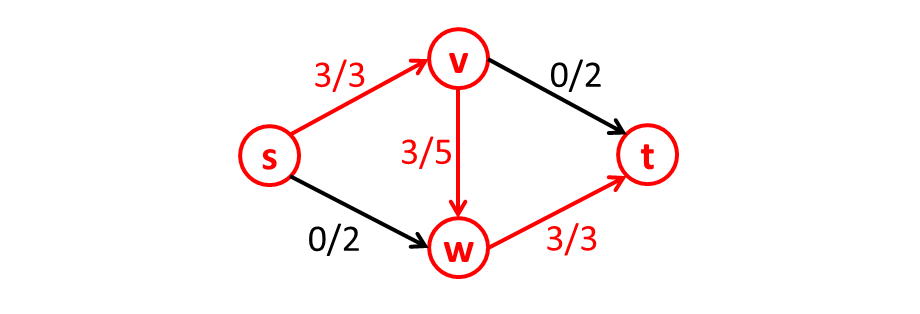
\includegraphics[width=0.8\linewidth]{1.png}\\
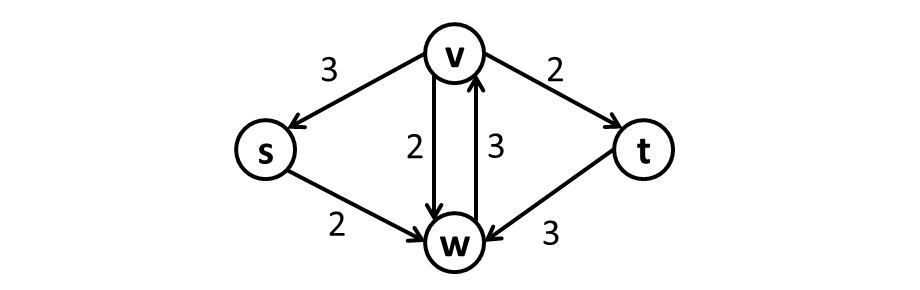
\includegraphics[width=0.8\linewidth]{2.png}
\end{figure}
\end{frame}

\subsection{Cammino aumentante}

\begin{frame}
\frametitle{Il metodo di Ford-Fulkerson\\Cammino aumentante}
Data una rete di flusso $G$ e un flusso $f$, un \textbf{cammino aumentante} è un cammino semplice che va da $s$ a $t$ nella rete residua $G_f$.\\
Dato un cammino aumentante $p$, chiamiamo \textbf{capacità residua} di $p$ la massima quantità di flusso che è possibile mandare su questo cammino:\\
$c_f(p)=min\{c_f(u,v):(u,v) \mbox{ sta in } p\}$.\\
Definiamo inoltre una funzione $f_p:V\times V\rightarrow \mathbb{R}$ nel seguente modo:\\
$$f_p(u,v) =
\left\{
	\begin{array}{ll}
		c_f(p) & \mbox{se } (u,v) \mbox{ sta in } p\\
		0 & \mbox{altrimenti}
	\end{array}
\right.$$\\
\begin{block}{Lemma}
$f_p$ è un flusso in $G_f$ di valore $|f_p|=c_f(p)>0$.
\end{block}
\begin{block}{Corollario}
$f\uparrow f_p$ è un flusso in $G$ di valore $|f\uparrow f_p|=|f|+|f_p|>|f|.$
\end{block}
\end{frame}

\subsection{Taglio}

\begin{frame}
\frametitle{Il metodo di Ford-Fulkerson\\Taglio}
Un \textbf{taglio} $(S,T)$ di una rete di flusso $G=(V,E)$ è una partizione di $V$ in $S$ e $T$ tale che $s\in S$ e $t\in T$.\\
Dato $f$ flusso, esprimiamo con $f(S,T)$ il \textbf{flusso che attraversa il taglio}:
$$f(S,T)=\sum\limits_{u\in S}\sum\limits_{v\in T}f(u,v)-
         \sum\limits_{u\in S}\sum\limits_{v\in T}f(v,u)$$
La \textbf{capacità di un taglio} $(S,T)$ è:
$$c(S,T)=\sum\limits_{u\in S}\sum\limits_{v\in T}c(u,v)$$
Il \textbf{taglio minimo} è il taglio di capacità minima fra i tagli della rete.
\end{frame}

\begin{frame}
\frametitle{Il metodo di Ford-Fulkerson\\Taglio}
\begin{block}{Lemma}
Dati $f$ flusso in $G$ con $s$ sorgente e $t$ pozzo, e (S,T) un qualsiasi taglio di $G$, il flusso attraverso $(S,T)$ è $f(S,T)=|f|$.
\end{block}
\begin{block}{Corollario}
Il valore di qualsiasi flusso $f$ su una rete $G$ è limitato superiormente dalla capacità di un qualsiasi taglio di $G$.
\end{block}
\begin{block}{Teorema del flusso massimo e taglio minimo}
Dati $f$ flusso in una rete $G=(V,E)$ con $s$ sorgente e $t$ pozzo, le seguenti condizioni sono equivalenti:
\begin{itemize}
\item $f$ è un flusso massimo in $G$
\item La rete residua $G_f$ non ammette cammini aumentanti
\item $|f|=c(S,T)$ per qualche taglio $(S,T)$ di $G$
\end{itemize}
\end{block}
\end{frame}

\subsection{Complessità}

\begin{frame}
\frametitle{Il metodo di Ford-Fulkerson\\Pseudocodice}
\begin{algorithm}[H]
    \caption{Ford-Fulkerson(G,s,t)}%\label{euclid}
    \begin{algorithmic}[1]
        \State \textbf{for} each edge $(u,v)\in E$
        \State \ \ \ \ \ \ $(u,v).f = 0$
        \State \textbf{while} esiste un cammino aumentante $p$ in $G_f$
        \State \ \ \ \ \ \ $c_f(p)=min\ \{c_f(u,v):(u,v)\mbox{ sta in }p\}$
        \State \ \ \ \ \ \ \textbf{for} each edge $(u,v)$ in $p$
        \State \ \ \ \ \ \ \ \ \ \ \ \ \textbf{if} $(u,v)\in E$
        \State \ \ \ \ \ \ \ \ \ \ \ \ \ \ \ \ \ \ $(u,v).f = (u,v).f + c_f(p)$
        \State \ \ \ \ \ \ \ \ \ \ \ \ \textbf{else}
        \State \ \ \ \ \ \ \ \ \ \ \ \ \ \ \ \ \ \ $(v,u).f = (v,u).f - c_f(p)$
    \end{algorithmic}
    \label{alg_1}
\end{algorithm}
\end{frame}

\begin{frame}
\frametitle{Il metodo di Ford-Fulkerson\\Complessità}
Una possibile implementazione del metodo consiste nello scegliere il cammino aumentante alla linea 3 in maniera arbitraria: l'algoritmo che si ottiene termina sempre a patto che le capacità degli archi siano valori razionali.\\
Per il caclolo della complessità, possiamo ridurci al caso in cui le capacità prendono valori interi.\\
Il ciclo \textbf{for} alle linee 1-2 ha complessità $O(|E|)$.\\
Se chiamiamo $f^*$ il flusso massimo, abbiamo che il ciclo \textbf{while} alla linea 3 verrà eseguito al più $|f^*|$ volte (ad ogni iterazione il valore del flusso aumenterà almeno di una unità). Trovare un cammino nella rete residua costa $O(|V|+|E|)=O(|E|)$ con BFS o DFS.\\
La complessità dell'algoritmo è quindi $O(|E|\cdot|f^*|)$. L'algoritmo è pseudopolinomiale.
\end{frame}

\begin{frame}
\frametitle{Il metodo di Ford-Fulkerson\\Caso pessimo}
Le prime tre immagini mostrano il primo passo dell'algoritmo e la successiva selezione del cammino aumentante. L'ultima immagine mostra lo stato al quale si arriva dopo 2000 iterazioni.
\begin{figure}
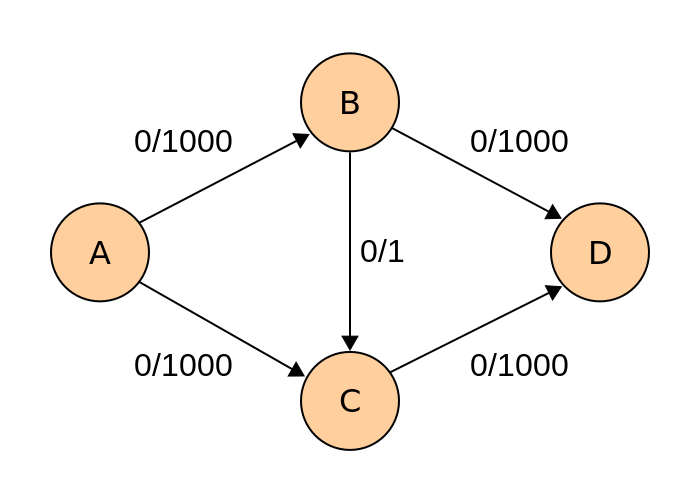
\includegraphics[width=0.3\linewidth]{11.png}
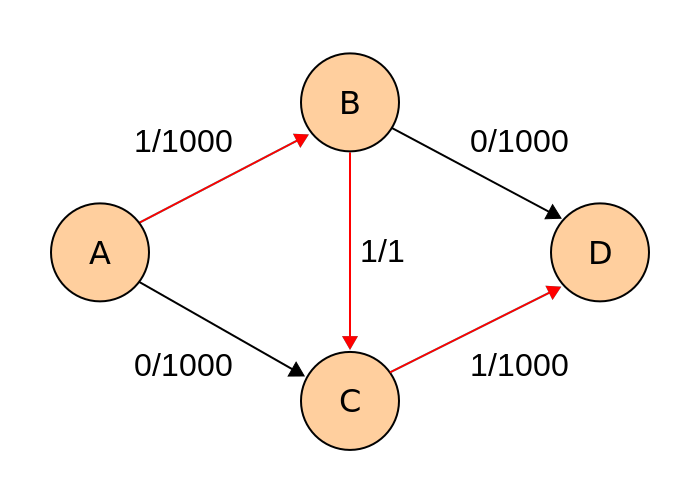
\includegraphics[width=0.3\linewidth]{12.png}\\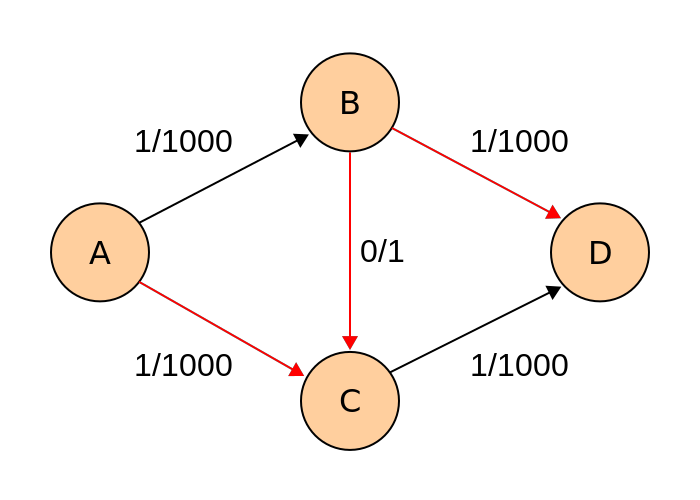
\includegraphics[width=0.3\linewidth]{13.png}
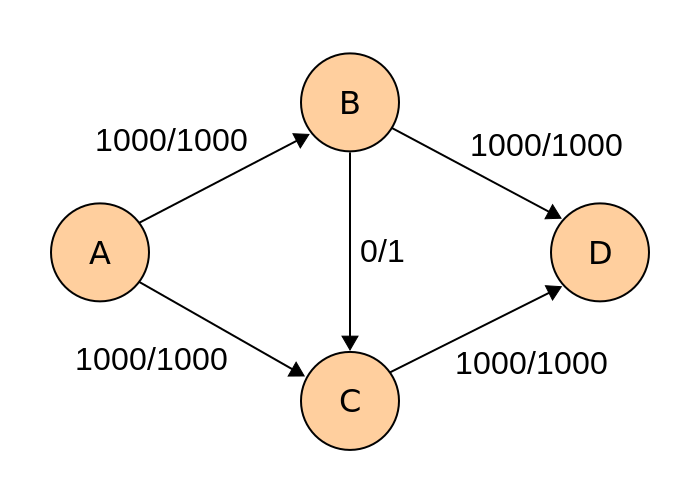
\includegraphics[width=0.3\linewidth]{14.png}
\end{figure}
\end{frame}

\section{L'algoritmo di Edmonds-Karp}

\subsection{Algoritmo}

\begin{frame}
\frametitle{L'algoritmo di Edmonds-Karp}
L'algoritmo di Edmonds-Karp è un'implementazione del metodo di Ford-Fulkerson che ci permette di risolvere il problema del massimo flusso in tempo $O(|V|\cdot|E|^2)$. L'algoritmo utilizza una ricerca in ampiezza per trovare, ad ogni iterazione, il \textbf{cammino minimo} da $s$ a $t$ nella rete residua.
\begin{block}{Lemma}
Dato $G=(V,E)$ con $s$ sorgente e $t$ pozzo, per tutti i $v\in V\setminus\{s,t\}$ abbiamo che la lunghezza del cammino minimo $\delta_f(s,v)$ fra $s$ e $v$ nella rete residua $G_f$ aumenta monotonicamente durante l'esecuzione dell'algoritmo.
\end{block}
\end{frame}

\subsection{Complessità}

\begin{frame}
\frametitle{L'algoritmo di Edmonds-Karp}
\begin{block}{Dimostrazione}
Supponiamo, per assurdo, che esista un vertice $v\in V\setminus\{s,t\}$ per il quale, in corrispondenza di un aumento del flusso, la distanza da $s$ si riduca. Chiamiamo $f$ il flusso prima di questo aumento, e $f'$ il flusso risultante. Sia $v$ il nodo tale che $\delta_{f'}(s,v)<\delta_f(s,v)$ e per il quale $\delta_{f'}(s,v)$ è minima. Sia inoltre $p=s\leadsto u\rightarrow v$ un cammino minimo da $s$ a $v$ in $G_{f'}$.\\
Abbiamo $\delta_{f'}(s,u)=\delta_{f'}(s,v)-1$.\\
Per come abbiamo scelto $v$, sappiamo inoltre che $\delta_{f'}(s,u)\geq \delta_f(s,u)$.\\
Se $(u,v)\in E_{f}$ avremmo:\\
$\delta_f(s,v)\ \leq\ \delta_f(s,u)+1$\ \ \ (disuguaglianza triangolare)\\
$\ \ \ \ \ \ \ \ \ \ \ \leq\ \delta_{f'}(s,u)+1$\\
$\ \ \ \ \ \ \ \ \ \ \ =\ \delta_{f'}(s,v)$\\
è una contraddizione, quindi $(u,v)\not\in E_f$.
\end{block}
\end{frame}

\begin{frame}
\frametitle{L'algoritmo di Edmonds-Karp}
\begin{block}{Dimostrazione}
Abbiamo mostrato che $(u,v)\not\in E_f$, sappiamo inoltre che $(u,v)\in E_{f'}$. Questo significa che l'aumento di flusso deve aver aumentato il flusso da $v$ a $u$.\\
L'algoritmo che stiamo analizzando aumenta sempre il flusso sul cammino minimo, quindi il cammino minimo da $s$ a $u$ in $G_f$ ha $(v,u)$ come ultimo arco. Abbiamo quindi:\\
$\delta_f(s,v)\ =\ \delta_f(s,u)-1$\\
$\ \ \ \ \ \ \ \ \ \ \ \leq\ \delta_{f'}(s,u)-1$\\
$\ \ \ \ \ \ \ \ \ \ \ =\ \delta_{f'}(s,v)-2$\\
Questo contraddice la nostra assunzione iniziale, cioè $\delta_{f'}(s,v)<\delta_f(s,v)$. Non esiste quindi un nodo $v$ con queste caratteristiche.
\end{block}
\end{frame}

\begin{frame}
\frametitle{L'algoritmo di Edmonds-Karp}
\begin{block}{Teorema}
Data una rete di flusso $G=(V,E)$, l'algoritmo di Edmonds-Karp aumenta il valore del flusso $O(|V|\cdot|E|)$ volte.
\end{block}
\begin{block}{Dimostrazione}
Un arco $(u,v)$ appartenente ad un cammino aumentante è \textbf{critico} se $c_f(p)=c_f(u,v)$. Quando aumentiamo il flusso, tutti gli archi critici appartenenti al cammino aumentante scompaiono dalla rete residua (inoltre, ogni cammino aumentante ha almeno un arco critico).\\
Quello che mostriamo è che ogni arco può diventare critico al più $|V|/2$ volte.
\end{block}
\end{frame}

\begin{frame}
\frametitle{L'algoritmo di Edmonds-Karp}
\begin{block}{Dimostrazione}
Siano $u,v$ nodi in $V$ tali che $(u,v)\in E$. Quando $(u,v)$ diventa critico per la prima volta, avremo $\delta_f(s,v)=\delta_f(s,u)+1$.\\
Dopo aver aumentato il flusso, l'arco $(u,v)$ scomparirà dalla rete residua.\\
Per far sì che $(u,v)$ ricompaia su un altro cammino aumentante, il flusso da $u$ a $v$ deve diminuire, cosa che succede solamente quando $(v,u)$ compare su un cammino aumentante.\\
Sia $f'$ un flusso tale che $(v,u)$ compare su un cammino aumentante.\\
Abbiamo:\\
$\delta_{f'}(s,u)\ =\ \delta_{f'}(s,v)+1$\\
$\ \ \ \ \ \ \ \ \ \ \ \ \geq\ \delta_{f}(s,v)+1$\ \ \ \ (Lemma)\\
$\ \ \ \ \ \ \ \ \ \ \ \ =\ \delta_{f}(s,u)+2$\\
Questo dimostra che da quando $(u,v)$ diventa critico al successivo momento in cui sarà critico, la distanza da $s$ ad $u$ aumenterà almeno di 2.
\end{block}
\end{frame}

\begin{frame}
\frametitle{L'algoritmo di Edmonds-Karp}
\begin{block}{Dimostrazione}
I nodi intermedi di un cammino minimo da $s$ a $u$ non possono mai contenere $s$, $u$ o $t$. Quindi, la distanza di $u$ (dopo ogni iterazione) sarà al più $|V|-2$.\\
Dopo che $(u,v)$ è diventato critico per la prima volta, può ridiventarlo al più altre $(|V|-2)/2=|V|/2-1$ volte, per un totale di $|V|/2$ volte.\\
Visto che il numero di archi che possono comparire in una rete residua è $O(|E|)$, il numero totale di archi critici durante l'esecuzione dell'algoritmo sarà $O(|V|\cdot|E|)$
\end{block}
Come visto precedentemente, possiamo individuare un cammino aumentante utilizzando BFS in tempo $O(|E|)$. La complessità dell'algoritmo è quindi
 $O(|V|\cdot|E|^2)$.
\end{frame}

\section{Algoritmi push-relabel}

\subsection{Algoritmo generico}

\begin{frame}
\frametitle{Algoritmi push-relabel\\Algoritmo generico}
L'approccio \textbf{push-relabel} consente di risolvere il problema del massimo flusso più velocemente rispetto all'approccio di Edmonds-Karp: arriveremo ad un algoritmo di complessità $O(|V|^3)$, uno degli algoritmi più veloci per questo tipo di problema.\\
Gli algoritmi push-relabel mantengono durante l'esecuzione il vincolo di capacità ma rilassano il vincolo di conservazione del flusso: richiediamo solamente che la quantità di flusso uscente da un nodo (fatta eccezione per sorgente e pozzo) non superi la quantità di flusso entrante:\\
$\sum\limits_{v\in V}f(v,u)-\sum\limits_{v\in V}f(u,v)\geq 0$\\
Chiamiamo inoltre \textbf{eccesso di flusso} la seguente quantità:\\
$e(u)=\sum\limits_{v\in V}f(v,u)-\sum\limits_{v\in V}f(u,v)$\\
L'idea alla base di questi algoritmi consiste nell'assegnare ad ogni nodo un'altezza, e fare in modo che un nodo $u$ possa aumentare il flusso su un arco $(u,v)$ solamente se $v$ sta ``più in basso".
\end{frame}

\begin{frame}
\frametitle{Algoritmi push-relabel\\Algoritmo generico}
\begin{itemize}
\item Inizialmente, alla sorgente assegnamo altezza $|V|$ mentre al pozzo e a tutti gli altri nodi assegnamo 0.
\item Assegnamo più flusso possibile agli archi uscenti dalla sorgente e avremo uno o più nodi del grafo aventi eccesso di flusso positivo.
\item Scelto uno di questi nodi ($u$), aumentiamo la sua altezza in modo che superi di 1 l'altezza del ``più basso" dei suoi vicini ($v$) scelto in modo che sia possibile aumentare il flusso su $(u,v)$. A questo punto possiamo assegnare del flusso ad almeno un arco uscente dal nodo $u$.
\item Iterando queste operazioni, arriveremo ad un punto nel quale il pozzo riceve la massima quantità di flusso possibile. Il flusso non è però legale visto che (in generale) può violare il vincolo di conservazione.
\item Per renderlo legale permettiamo che l'altezza dei nodi possa superare $|V|$. In questo modo, il flusso in eccesso viene ``spinto" di nuovo alla sorgente (cancellazione) e otteniamo un flusso vero e proprio (legale e massimo).
\end{itemize}
\end{frame}

\begin{frame}
\frametitle{Algoritmi push-relabel\\Algoritmo generico}
Quando $u.e>0$, $c_f(u,v)>0$ e $u.h=v.h+1$ possiamo eseguire un'operazione di Push:
\begin{algorithm}[H]
    \caption{Push(u,v)}%\label{euclid}
    \begin{algorithmic}[1]
        \State $\Delta_f(u,v)=min(u.e,c_f(u,v))$
        \State \textbf{if} $(u,v)\in E$
        \State \ \ \ \ \ \ $(u,v).f = (u,v).f+\Delta_f(u,v)$
        \State \textbf{else}
        \State \ \ \ \ \ \ $(v,u).f = (v,u).f-\Delta_f(u,v)$
        \State $u.e=u.e-\Delta_f(u,v)$
        \State $v.e=v.e+\Delta_f(u,v)$
    \end{algorithmic}
    \label{alg_1}
\end{algorithm}
La linea 5 corrisponde ad una diminuzione del flusso sull'arco (v,u). Questo accade quando $(u,v)$ fa parte della rete residua ma non della rete originale.
\end{frame}

\begin{frame}
\frametitle{Algoritmi push-relabel\\Algoritmo generico}
Quando $u.e>0$ e per ogni $(u,v)\in E_f$ si ha $u.h\leq v.h$, possiamo eseguire un'operazione di Relabel:
\begin{algorithm}[H]
    \caption{Relabel(u)}%\label{euclid}
    \begin{algorithmic}[1]
        \State $u.h=1+min\{v.h:(u,v)\in E_f\}$
    \end{algorithmic}
    \label{alg_1}
\end{algorithm}
La precondizione è sufficiente a garantire che esista almeno un arco uscente da $u$ nella rete residua:\\
$u.e>0$ implica l'esistenza di almeno un nodo $v$ tale che $(v,u).f>0$,  quindi $c_f(u,v)>0$ che a sua volta implica $(u,v)\in E_f$.
\end{frame}

\begin{frame}
\frametitle{Algoritmi push-relabel\\Algoritmo generico}
\begin{algorithm}[H]
    \caption{Initialize(G,s)}%\label{euclid}
    \begin{algorithmic}[1]
        \State \textbf{for} each vertex $v\in V$
        \State \ \ \ \ \ \ $v.h=0$
        \State \ \ \ \ \ \ $v.e=0$
        \State $s.h=|V|$
        \State \textbf{for} each $(u,v)\in E$
        \State \ \ \ \ \ \ $(u,v).f=0$
        \State \textbf{for} each vertex $v\in s.Adj$
        \State \ \ \ \ \ \ $(s,v).f=c(s,v)$
        \State \ \ \ \ \ \ $v.e=c(s,v)$
        %\State \ \ \ \ \ \ $s.e=s.e-c(s,v)$
    \end{algorithmic}
    \label{alg_1}
\end{algorithm}
%La linea 10 serve ad impedire che l'algoritmo inizi a ciclare scegliendo $s$ come nodo dal quale effettuare operazioni di push.
\end{frame}

\begin{frame}
\frametitle{Algoritmi push-relabel\\Algoritmo generico}
\begin{algorithm}[H]
    \caption{Generic-push-relabel(G)}%\label{euclid}
    \begin{algorithmic}[1]
        \State Initialize(G,s)
        \State \textbf{while} esiste un'operazione Push o Relabel applicabile
        \State \ \ \ \ \ \ seleziona un'operazione ed eseguila
    \end{algorithmic}
    \label{alg_1}
\end{algorithm}
E' possibile mostrare che questo algoritmo ha complessità asintotica pari a $O(|V|^2\cdot|E|)$.
\end{frame}

\subsection{Algoritmo relabel-to-front}

\begin{frame}
\frametitle{Algoritmi push-relabel\\Algoritmo relabel-to-front}
L'algoritmo \textbf{relabel-to-front} è un algoritmo push-relabel nel quale viene specificato l'ordine con il quale applicare le operazioni di base (Push e Relabel) tramite un'opportuna struttura dati.\\
Questo accorgimento permette di ottenere una complessità pari a $O(|V|^3)$ (l'algoritmo generico ha complessità $O(|V|^2\cdot|E|)$).\\
Una \textbf{Neighbor List} $u.N$ per il nodo $u$ è una linked list contenente (tutti) i vicini di $u$ (tutti i nodi tali che $(u,v)\in E$ oppure $(v,u)\in E$).\\
Con l'attributo $u.N.head$ puntiamo al primo elemento della lista mentre $v.next\mbox{-}neighbor$ punta all'elemento che segue $v$ all'interno della lista.\\
$u.current$ punta al nodo che sto attualmente analizzando in $u.N$.
\end{frame}

\begin{frame}
\frametitle{Algoritmi push-relabel\\Algoritmo relabel-to-front}
\begin{algorithm}[H]
    \caption{Discharge(u)}%\label{euclid}
    \begin{algorithmic}[1]
        \State \textbf{while} $u.e>0$
        \State \ \ \ \ \ \ $v=u.current$
        \State \ \ \ \ \ \ \textbf{if} $v==NIL$
        \State \ \ \ \ \ \ \ \ \ \ \ \ Relabel(u)
        \State \ \ \ \ \ \ \ \ \ \ \ \ $u.current=u.N.head$
        \State \ \ \ \ \ \ \textbf{elseif} $c_f(u,v)>0\ \wedge\ u.h==v.h+1$
        \State \ \ \ \ \ \ \ \ \ \ \ \ Push(u,v)
        \State \ \ \ \ \ \ \textbf{else}
        \State \ \ \ \ \ \ \ \ \ \ \ \ $u.current=v.next\mbox{-}neighbor$
    \end{algorithmic}
    \label{alg_1}
\end{algorithm}
\end{frame}

\begin{frame}
\frametitle{Algoritmi push-relabel\\Algoritmo relabel-to-front}
Per definire l'algoritmo completo, utilizziamo un'ulterione lista $L$ contenente tutti i nodi eccetto sorgente e pozzo.
\begin{algorithm}[H]
    \caption{Relabel-to-front(G,s,t)}%\label{euclid}
    \begin{algorithmic}[1]
        \State Initialize(G,s)
        \State $L=V\setminus\{s,t\}$
        \State \textbf{for} each vertex $u\in V\setminus\{s,t\}$
        \State \ \ \ \ \ \ $u.current=u.N.head$
        \State $u=L.head$
        \State \textbf{while} $u\not =NIL$
        \State \ \ \ \ \ \ $old\mbox{-}height=u.h$
        \State \ \ \ \ \ \ Discharge(u)
        \State \ \ \ \ \ \ \textbf{if} $u.h>old\mbox{-}height$
        \State \ \ \ \ \ \ \ \ \ \ \ \ move $u$ to the front of $L$
        \State \ \ \ \ \ \ $u=u.next$
    \end{algorithmic}
    \label{alg_1}
\end{algorithm}
\end{frame}

\subsection{Complessità}

\begin{frame}
\frametitle{Algoritmi push-relabel\\Complessità}
\begin{block}{Lemma}
Il numero totale di operazioni \textbf{relabel} che eseguiamo è al più $2|V|-1$ per ogni vertice. In totale è minore di $2|V|^2$.
\end{block}
\begin{block}{Lemma}
Il tempo totale che spendiamo per le operazioni di \textbf{relabel} è limitato da $O(|V|\cdot|E|)$.
\end{block}
\begin{block}{Lemma}
Durante l'esecuzione dell'algoritmo, il numero totale di operazioni di \textbf{push} tali che l'arco viene \textbf{saturato} è limitato superiormente da $|V|\cdot|E|$.
\end{block}
\end{frame}

\begin{frame}
\frametitle{Algoritmi push-relabel\\Complessità}
\begin{block}{Teorema}
L'algoritmo relabel-to-front ha complessità $O(|V|^3)$.
\end{block}
\begin{block}{Dimostrazione}
Poniamo un bound al numero di volte che \textbf{discharge} viene chiamato. Sappiamo che $O(|V|^2)$ è un bound per il numero delle operazioni \textbf{relabel}. Mostriamo che per ogni coppia di \textbf{relabel} consecutivi, abbiamo al più $|V|$ \textbf{discharge}: se \textbf{discharge} non esegue \textbf{relabel} andiamo avanti sulla lista $L$ che contiene $<|V|$ elementi, se invece esegue \textbf{relabel}, la chiamata successiva a \textbf{discharge} avverrà banalmente dopo il \textbf{relabel} stesso.\\
Concludiamo quindi che \textbf{discharge} può essere chiamato al più $O(|V|^3)$ volte.
\end{block}
\end{frame}

\begin{frame}
\frametitle{Algoritmi push-relabel\\Complessità}
\begin{block}{Dimostrazione}
Analizziamo ora la complessità della procedura \textbf{discharge}.\\
Ogni iterazione del ciclo while eseguirà una delle seguenti operazioni:\\
\begin{itemize}
\item \textbf{relabel}: in questo caso abbiamo un bound sul tempo totale richiesto per eseguire le operazioni \textbf{relabel}, $O(|V|\cdot|E|)$.
\item \textbf{push}: sappiamo che il numero totale di operazioni \textbf{push} tale che l'arco viene \textbf{saturato} è $O(|V|\cdot|E|)$. Quando eseguiamo una \textbf{push} ``non-saturante" usciamo immediatamente dalla chiamata a \textbf{discharge} (perchè non è più presente flusso in eccesso) quindi questo tipo di \textbf{push} verrà eseguito in totale $O(|V|^3)$ volte.
\item \textbf{aggiornamento} di $u.current$: ogni volta che su un nodo $u$ viene eseguito un \textbf{relabel}, abbiamo $O(grado(u))$ aggiornamenti del puntatore. Utilizzando l'uguaglianza \small$\sum\limits_{v\in V}$ $grado(v)=2|E|$ e il bound al numero di relabel di un vertice $O(|V|)$, otteniamo $O(|V|\cdot|E|)$.
\end{itemize}

\end{block}
\end{frame}

\begin{frame}
\frametitle{Algoritmi push-relabel\\Complessità}
\begin{block}{Dimostrazione}
La complessità totale risulta quindi essere $O(|V|^3+|V|\cdot|E|)=O(|V|^3)$.
\end{block}
\end{frame}

\end{document}